% 1999 年全国卷文科第 22 题：正四棱柱中的截面 EAC
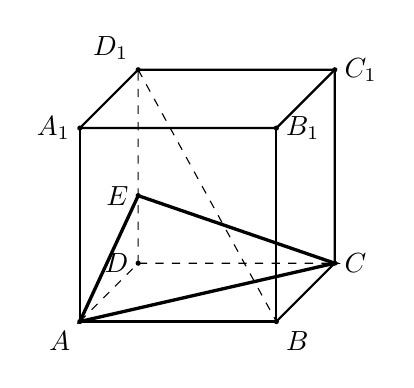
\begin{tikzpicture}[scale=0.78, >=stealth]
  \coordinate (A)  at (0,0);
  \coordinate (B)  at (3.2,0);
  \coordinate (C)  at (4.15,0.95);
  \coordinate (D)  at (0.95,0.95);
  \coordinate (A1) at (0,3.15);
  \coordinate (B1) at (3.2,3.15);
  \coordinate (C1) at (4.15,4.1);
  \coordinate (D1) at (0.95,4.1);
  \coordinate (E)  at (0.95,2.05);

  \draw[thick] (A)--(B)--(B1)--(A1)--cycle;
  \draw[thick] (A1)--(B1)--(C1)--(D1)--cycle;
  \draw[thick] (B)--(C)--(C1);
  \draw[dashed] (A)--(D)--(C) (D)--(D1) (A1)--(D1);
  \draw[dashed] (D1)--(B);
  \draw[very thick] (A)--(E)--(C)--cycle;

  \fill (A)  circle (1.2pt) node[below left] {$A$};
  \fill (B)  circle (1.2pt) node[below right] {$B$};
  \fill (C)  circle (1.2pt) node[right] {$C$};
  \fill (D)  circle (1.2pt) node[left] {$D$};
  \fill (A1) circle (1.2pt) node[left] {$A_1$};
  \fill (B1) circle (1.2pt) node[right] {$B_1$};
  \fill (C1) circle (1.2pt) node[right] {$C_1$};
  \fill (D1) circle (1.2pt) node[above left] {$D_1$};
  \fill (E)  circle (1.2pt) node[left] {$E$};
\end{tikzpicture}
